\documentclass{article}
\usepackage{graphicx} % Required for inserting images
\usepackage[utf8]{inputenc}
\usepackage{amsmath}
\usepackage{graphicx}
\usepackage{tikz}
\usepackage{array}
\usetikzlibrary{trees}
\usepackage{amssymb}
\usepackage{amsthm}
\usepackage{multirow}
\usepackage{dcolumn}
\usepackage{verbatim}
\usepackage{booktabs}
\usepackage{listings}
\usepackage{array}
\usepackage{xcolor}

\newcolumntype{2}{D{.}{}{2.0}}

\title{CSC279 HW5}
\author{Hanzhang Yin}
\date{Nov/22/2023}

\begin{document}

\maketitle

\lstset{ 
    language=Python, % Specify language
    basicstyle=\ttfamily\footnotesize, % Font style
    keywordstyle=\color{blue}, % Keywords color
    commentstyle=\color{green!60!black}, % Comment color
    stringstyle=\color{red}, % String color
    numbers=left, % Line numbers on the left
    numberstyle=\tiny\color{gray}, % Line number style
    stepnumber=1, % Number every line
    numbersep=5pt, % Line number separation
    showstringspaces=false, % Don't show spaces in strings
    breaklines=true, % Break lines if necessary
    frame=single, % Frame around code
    captionpos=b, % Caption position (b for bottom)
    tabsize=4, % Tab size
}

\subsection*{Collaborator}
Chenxi Xu, Yekai Pan, Yiling Zou, Boyi Zhang

\subsection*{PROBLEM 15}
\\
\textbf{Answer: }

\begin{enumerate}
    \item Assume $q$ is inside $P$. We want to find the closest point to $q$ in $\{p_1, \dots, p_n\}$.
    \\
    \textbf{Reasoning: }
    \\
    Hard and required $\Omega(n)$ runtime. Arrange all points on the circumference of a circle like regular convex n-polygon enclosing point $q$ as its center. 
    If the algorithm is deterministic and assumes an easy case, some points remain unvisited. For those unvisited point, we one of them closer.
    Therefore, the algorithm can not find the correct closest point and outputting incorrect results.
    \item Assume $q$ is outside $P$. We want to find the closest point to $q$ in $\{p_1, \dots, p_n\}$.
    \\
    \textbf{Reasoning: }
    \\
    Hard and required $\Omega(n)$ runtime. Place all points on a quarter-circle like regular convex n-polygon enclosing point $q$ while ensuring $P$ is convex and non-enclosing.
    Assume easy, then there will be some point that the algorithm (deterministic) will not visit. For an unvisited point, we move it closer. 
    Therefore, the algorithm can not find the correct closest point and outputting incorrect results.
    \item Assume $q$ is inside $P$. We want to find the farthest point to $q$ in $\{p_1, \dots, p_n\}$.
    \\
    \textbf{Reasoning: }
    \\
    Hard and required $\Omega(n)$ runtime. Similar to Q1, but this time we move an unvisited point further.
    \item Assume $q$ is outside $P$. We want to find the farthest point to $q$ in $\{p_1, \dots, p_n\}$.
    \\
    \textbf{Reasoning: }
    \\
    Hard and required $\Omega(n)$ runtime. Similar to Q2, but this time we move an unvisited point further.
    \item Assume $q$ is inside $P$. We want to find the closest point to $q$ on $P$.
    \\
    \textbf{Reasoning: }
    \\
    Hard and required $\Omega(n)$ runtime. Similar to Q1 again, The number of edges equals the number of points, so we still need at least $O(n)$ runtime.
    \item Assume $q$ is outside $P$. We want to find the closest point to $q$ on $P$.
    \\
    \textbf{Reasoning: }
    \\
    Easy and can be solved within $O(logn)$. 
    \\
    The algorithm finds the closest point to \( q \) on a convex polygon \( P \) in \( O(\log n) \) time using the unimodal nature of the distance function from \( q \) to \( P \). 
    Using ternary search on the edges of \( P \), it narrows the search interval until the closest edge is identified, and then computes the closest point on that edge. 
    The convexity of \( P \) ensures the unimodal property, guaranteeing the correctness of the ternary search.
    
    \begin{verbatim}
        def closest_point_on_convex_polygon(q, P):
            n = len(P)
            low = 0
            high = n - 1

        while high - low > 3:
            m1 = low + (high - low) // 3
            m2 = high - (high - low) // 3

            D_m1 = distance_to_edge(q, P[m1], P[(m1 + 1) % n])
            D_m2 = distance_to_edge(q, P[m2], P[(m2 + 1) % n])

            if D_m1 < D_m2:
                high = m2
            else:
                low = m1

        min_dist = float('inf')
        closest_point = None

        for i in range(low, high + 1):
            p1 = P[i]
            p2 = P[(i + 1) % n]
            c = closest_point_on_segment(q, p1, p2)
            D = distance(q, c)
            if D < min_dist:
                min_dist = D
                closest_point = c

        return closest_point
    \end{verbatim}
    \item Assume $q$ is inside $P$. We want to find the farthest point to $q$ on $P$.
    \\
    \textbf{Reasoning: }
    \\
    Hard and required $\Omega(n)$ runtime. Similar to Q3, so similar argument can be made.
    \item Assume $q$ is outside $P$. We want to find the farthest point to $q$ on $P$.
    \\
    \textbf{Reasoning: }
    \\
    Hard and required $\Omega(n)$ runtime. Similar to Q4. The farthest point must lie on the circumcircle as all other points are on an n-gon, so similar argument can be made.
\end{enumerate}

\newpage

\subsection*{PROBLEM 16}

\begin{proof}
    \textbf{Theorem: }
    \\
    A convex polygon is fully contained within the largest circumcircle formed by three of its consecutive vertices.
    \\
    \textbf{Lemma: }
    \\
    Let \( P = \{p_1, p_2, \ldots, p_n\} \) represent a convex polygon. Suppose a triangle \( T \) is formed by three vertices of \( P \), and the circumcircle of \( T \) contains \( P \). For any edge \( \overline{p_a p_b} \) of \( T \), there exists a vertex \( p_c \) between \( p_a \) and \( p_b \) such that the circumcircle of \( T_{ab,c} \) contains \( P \).
    \\
    \textbf{Proof}
    \\
    Let \( p_i, p_j, p_k \) be three vertices defining the triangle \( T_{ij,k} \). Without loss of generality, consider the edge \( \overline{p_jp_k} \) and its corresponding arc on the circumcircle. There exists \( c \in (i, j) \) such that for every \( a \in (i, j) \), the circumcircle of \( T_{ij,c} \) contains \( p_a \).
    \\
    Now, we examine two cases for \( p_c \):
    \\
    \textbf{Case 1: \( p_c \) lies on the circumcircle of \( T_{ij,k} \)}
    If \( p_c \) is on the circumcircle of \( T_{ij,k} \), then the circumcircle of \( T_{j,k,c} \) is the same as that of \( T_{ij,k} \). Thus, the lemma holds.
    \\
    \textbf{Case 2: \( p_c \) lies inside the circumcircle of \( T_{ij,k} \)}
    \begin{figure*}[h]
        \centering
        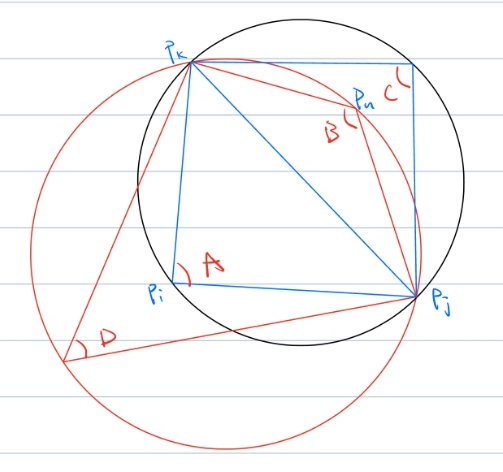
\includegraphics[width=0.9\textwidth]{HW5_Q2_Proof_Helper_Graph.png}
        \label{fig:q2_proof}
    \end{figure*}
    Construct a quadrilateral with vertices \( p_j, p_c, p_k, D \) that forms a cyclic quadrilateral. By the properties of cyclic quadrilaterals:
    \[
        \angle A + \angle D = \pi \quad \text{and} \quad \angle B + \angle C = \pi.
    \]
    Using these properties:
    \[
        \angle A + \angle B = \pi - \angle C < \pi - \angle D \implies \angle A > \angle D.
    \]
    For any point \( z \) inside or on the circumcircle of $T_{i,j,k}$, it cannot satisfy \( \angle p_j z p_k > \angle p_j p_i p_k \). Thus, \( z \) must lie outside the circumcircle of \( T_{ij,k} \), ensuring that the circumcircle of \( T_{ij,c} \) contains all points between the arc \( p_j p_i p_k \). Hence, the lemma is proved.
    \\
    \textbf{Triangulation Construction}
    \begin{enumerate}
        \item Start with three consecutive vertices \( p_i, p_{i+1}, p_{i+2} \) such that the circumcircle of \( T_{p_i p_{i+1} p_{i+2}} \) contains \( P \).
        \item For each new triangle \( T \), select any edge \( \overline{p_a p_b} \). If there are no points of \( P \) within the range of vertices \( \overline{p_a p_b} \), skip this edge. Otherwise, find a point \( p_c \) such that the circumcircle of \( T_{p_a p_b p_c} \) contains \( P \).
        \item Repeat this process iteratively, ensuring that every newly constructed triangle satisfies the condition that its circumcircle contains \( P \).
    \end{enumerate}
    \\
    This method guarantees that the entire polygon \( P \) is contained within the circumcircle of the final triangulation.
\end{proof}

\newpage

\subsection*{PROBLEM 17}

\subsubsection*{General Algorithm Thoughts: }
\begin{enumerate}
    \item \textbf{Construct the Voronoi diagram} for all sites.
    \item \textbf{For each Voronoi cell}, examine its corners (vertices).
    \item \textbf{Check if any corner is at a distance} $\geq l + r$ \textbf{from its associated site}.
    \begin{itemize}
        \item \textbf{Reasoning}: Corners are the farthest points within a cell from the site.
        \item They are \textbf{equidistant to the site and neighboring sites}.
        \item If a corner is at distance $\geq l + r$ from the site, it is also that far from neighboring sites.
    \end{itemize}
    \item \textbf{Conclusion}: If such a corner exists, the site is "good" because all points at that corner are sufficiently distant from all relevant sites.
\end{enumerate}

\subsubsection*{Potentially A More Refined and Rigorous Version}
The algorithm identifies all "good" points by first constructing the Voronoi diagram of the given points, which efficiently captures proximity relationships in \( O(n \log n) \) time. 
For each point \( p_i \), it examines only its neighboring points in the Voronoi diagram, as these are the only ones that could potentially interfere with placing a new circle. By computing the angular intervals where a circle of radius \( \ell \) touching \( C_i \) would intersect any neighboring \( C_j \), 
the algorithm determines the directions that are blocked. If there exists at least one direction where such interference does not occur, the point \( p_i \) is therefore "good".

\begin{verbatim}
# Helper Functions
def compute_interfering_angles(p_i, p_j, r, l, d_ij):
    # Calculate the angle between p_i and p_j
    delta_x = p_j.x - p_i.x
    delta_y = p_j.y - p_i.y
    alpha = atan2(delta_y, delta_x)

    # Law of Cosines to find the angular width
    cos_theta = (d_ij**2 + (r + l)**2 - (r + l)**2) / (2 * d_ij * (r + l))
    if abs(cos_theta) <= 1:
        theta = acos(cos_theta)
        # The interfering interval is [alpha - theta, alpha + theta]
        interval = [(alpha - theta) % (2 * pi), (alpha + theta) % (2 * pi)]
        # Handle interval wrapping around 2pi
        if interval[0] > interval[1]:
            return [(interval[0], 2 * pi), (0, interval[1])]
        else:
            return [interval]
    else:
        # Circles do not intersect; no interfering angles
        return []

# Main Function
def find_good_points(P, r, l):
    # Construct the Voronoi diagram
    # Need O(nlogn)
    V = voronoi_diagram(P)

    good_points = []

    # For each point p_i
    # Need O(n)
    for p_i in P:
        interfering_angles = []  # List to store interfering angular intervals

        # Get neighboring points in the Voronoi diagram
        neighbors = V.get_neighbors(p_i)

        # For each neighbor p_j
        for p_j in neighbors:
            d_ij = distance(p_i, p_j)

            # Only consider neighbors that may interfere
            if d_ij < 2 * (r + l):
                # Compute the angular intervals of interference
                angles = compute_interfering_angles(p_i, p_j, r, l, d_ij)
                interfering_angles.extend(angles)

        # Compute the union of interfering intervals
        interfering_union = union_of_intervals(interfering_angles)

        # Determine the complement of the union over [0, 2pi)
        non_interfering_angles = complement_of_intervals(interfering_union, 0, 2 * pi)

        # If there is at least one non-interfering angle, p_i is good
        if non_interfering_angles:
            good_points.append(p_i)

    return good_points
\end{verbatim}

\newpage

\subsection*{PROBLEM 18}

\textbf{Summary: }
The randomized incremental Delaunay triangulation algorithm employs a history DAG to efficiently manage point insertion and triangle updates while ensuring the Delaunay property. 
The algorithm inserts points in random order, using the history DAG for \(O(\log n)\) expected-time point location, followed by triangle splitting and recursive edge flipping to maintain the Delaunay criterion. 
With an expected time complexity of \(O(n \log n)\) and space complexity of \(O(n \log n)\) (including the history DAG), it offers good average-case performance and practical simplicity.
\\
\textbf{Numerical Result: }
\\
\begin{table}[h!]
    \centering
    \begin{tabular}{@{}cccccc@{}}
    \toprule
    \textbf{Points} & \textbf{Grid} & \textbf{Max Depth} & \textbf{Avg Depth} & \textbf{Total Nodes} \\ \midrule
    25  & \(5 \times 5\)   & 9 & 5.66 & 63  \\
    100 & \(10 \times 10\) & 17 & 9.85 & 251  \\
    225 & \(15 \times 15\) & 19 & 11.08 & 563  \\
    400 & \(20 \times 20\) & 21 & 12.23 & 1001 \\
    \end{tabular}
    \caption{Depth and node statistics for randomized Delaunay triangulation on different grid sizes.}
    \label{tab:numerical-results}
    \end{table}

\begin{figure*}[h]
    \centering
    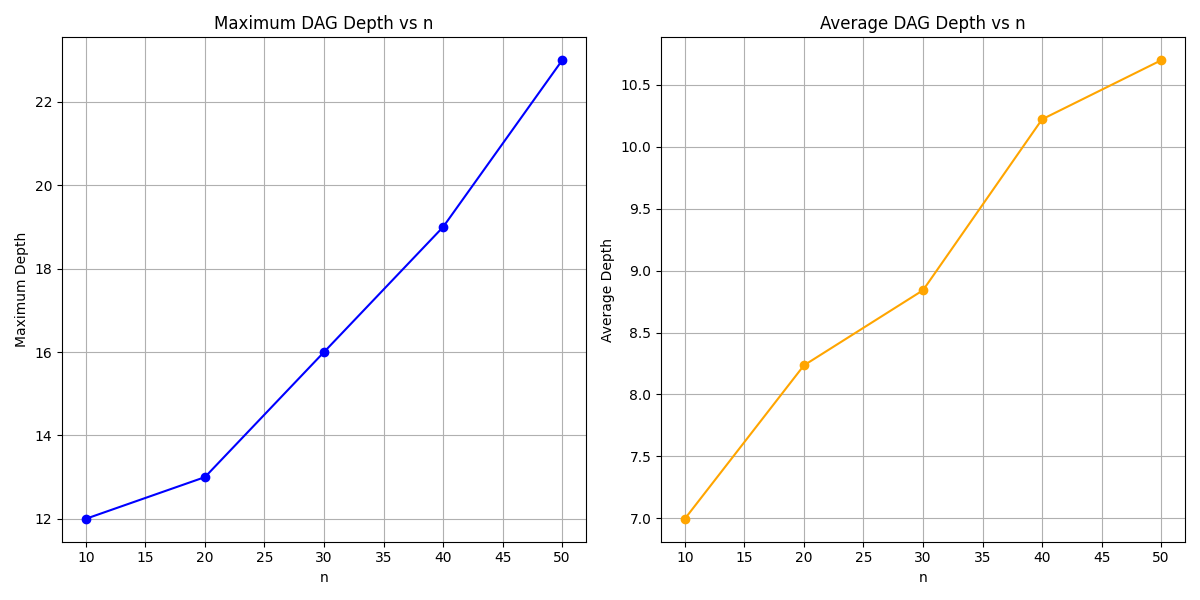
\includegraphics[width=0.9\textwidth]{Figure_1.png}
    \label{fig:model}
\end{figure*}

\hspace{0.01cm}
\\
\textbf{Short Analysis: }
\\
The result I got is reasonable, with the average depths increasing in $log n$ as expected, indicating that the algorithm effectively maintains a balanced DAG structure. 
Although the maximum depths are somewhat higher than theoretical predictions, they remain within an acceptable range considering the algorithm's randomness and the potential for local depth increases during edge legalization. 
\\
\textbf{Implementation: }
\\
The following code of randomized Delaunay triangulation algorithm with history DAG was implemented in Python (I fixed the random seed = 20 for better representation):
\begin{lstlisting}
import numpy as np
import matplotlib.pyplot as plt
from typing import List, Set, Tuple, Optional
from dataclasses import dataclass
import random
from collections import defaultdict

# Basic geometric structures
@dataclass
class Point2D:
    x: float
    y: float
    
    def __eq__(self, other):
        if not isinstance(other, Point2D):
            return False
        return abs(self.x - other.x) < 1e-10 and abs(self.y - other.y) < 1e-10
    
    def __str__(self):
        return f"Point2D({self.x:.2f}, {self.y:.2f})"

class Triangle2D:
    def __init__(self, points=None, p1=None, p2=None, p3=None):
        if points is not None:
            self.vertices = list(points)
        else:
            self.vertices = [p1, p2, p3]
    
    def get_points(self):
        return self.vertices
    
    def get_point(self, index):
        return self.vertices[index]
    
    def set_points(self, points=None, p1=None, p2=None, p3=None):
        if points is not None:
            self.vertices = list(points)
        else:
            self.vertices = [p1, p2, p3]

class DagNode:
    def __init__(self, triangle_index: int):
        self.triangle = triangle_index
        self.children = []
    
    def append_child(self, new_node):
        self.children.append(new_node)
    
    def get_index(self):
        return self.triangle
    
    def get_children(self):
        return self.children

class TriangulationMember(Triangle2D):
    def __init__(self, points, adj_list, dag_node, is_active=True):
        super().__init__(points)
        self.adj_list = list(adj_list)
        self.dag_node = dag_node
        self.active = is_active
    
    def set_active(self):
        self.active = True
    
    def set_inactive(self):
        self.active = False
    
    def is_active(self):
        return self.active
    
    def get_neighbour(self, index):
        return self.adj_list[index]
    
    def get_neighbours(self):
        return self.adj_list
    
    def get_dag_node(self):
        return self.dag_node
    
    def set_neighbour(self, neighbour, new_index):
        self.adj_list[neighbour] = new_index

class Triangulation:
    def __init__(self, init_triangle: Triangle2D, dag_node: DagNode):
        adj_list = [0, 0, 0]
        self.triangles = [TriangulationMember(init_triangle.get_points(), adj_list, dag_node)]
    
    def get_triangle(self, index):
        return self.triangles[index]
    
    def get_triangles(self):
        return self.triangles
    
    def size(self):
        return len(self.triangles)
    
    def add_triangle(self, triangle):
        self.triangles.append(triangle)
    
    def set_triangle_active(self, index):
        self.triangles[index].set_active()
    
    def set_triangle_inactive(self, index):
        self.triangles[index].set_inactive()
    
    def set_triangle_neighbour(self, triangle, neighbour, new_index):
        self.triangles[triangle].set_neighbour(neighbour, new_index)

# Geometric utilities
class GeometryUtils:
    @staticmethod
    def point_in_circle(p1: Point2D, p2: Point2D, p3: Point2D, p4: Point2D, include_edges: bool) -> bool:
        matrix = np.array([
            [p1.x - p4.x, p1.y - p4.y, (p1.x - p4.x)**2 + (p1.y - p4.y)**2],
            [p2.x - p4.x, p2.y - p4.y, (p2.x - p4.x)**2 + (p2.y - p4.y)**2],
            [p3.x - p4.x, p3.y - p4.y, (p3.x - p4.x)**2 + (p3.y - p4.y)**2]
        ])
        det = np.linalg.det(matrix)
        return det > 0 if include_edges else det >= 0

    @staticmethod
    def point_position_to_segment(p1: Point2D, p2: Point2D, p: Point2D) -> float:
        return (p2.x - p1.x) * (p.y - p1.y) - (p2.y - p1.y) * (p.x - p1.x)

    @staticmethod
    def point_in_triangle(p1: Point2D, p2: Point2D, p3: Point2D, p: Point2D, include_edges: bool) -> bool:
        pos1 = GeometryUtils.point_position_to_segment(p1, p2, p)
        pos2 = GeometryUtils.point_position_to_segment(p2, p3, p)
        pos3 = GeometryUtils.point_position_to_segment(p3, p1, p)
        
        if include_edges:
            return (pos1 >= 0 and pos2 >= 0 and pos3 >= 0) or (pos1 <= 0 and pos2 <= 0 and pos3 <= 0)
        else:
            return (pos1 > 0 and pos2 > 0 and pos3 > 0) or (pos1 < 0 and pos2 < 0 and pos3 < 0)

class DelaunayTriangulation:
    @staticmethod
    def update_index_in_neighbour(triangulation: Triangulation, triangle_index: int, 
                                neighbour_index: int, new_index: int):
        if neighbour_index != 0:
            neighbour = triangulation.get_triangle(neighbour_index)
            for i in range(3):
                if neighbour.get_neighbour(i) == triangle_index:
                    triangulation.set_triangle_neighbour(neighbour_index, i, new_index)

    @staticmethod
    def find_index_in_neighbour(triangulation: Triangulation, triangle_index: int, 
                                neighbour_index: int) -> int:
        for i in range(3):
            if triangulation.get_triangle(neighbour_index).get_neighbour(i) == triangle_index:
                return i
        return 3

    @staticmethod
    def flip_edge(triangulation: Triangulation, triangle_index: int, point_index: int):
        triangle = triangulation.get_triangle(triangle_index)
        
        if triangle.get_neighbour((point_index + 1) % 3) != 0:
            adj_triangle = triangulation.get_triangle(triangle.get_neighbour((point_index + 1) % 3))
            adj_point_index = (DelaunayTriangulation.find_index_in_neighbour(
                triangulation, triangle_index, 
                triangle.get_neighbour((point_index + 1) % 3)) + 2) % 3
            
            if GeometryUtils.point_in_circle(
                triangle.get_point(0), triangle.get_point(1), 
                triangle.get_point(2), adj_triangle.get_point(adj_point_index), False):
                
                triangulation.set_triangle_inactive(triangle_index)
                triangulation.set_triangle_inactive(triangle.get_neighbour((point_index + 1) % 3))
                
                current_index = triangulation.size()
                new_triangle_index1 = current_index
                new_triangle_index2 = current_index + 1
                
                # Create new triangles
                new_triangle1 = Triangle2D(
                    p1=triangle.get_point(point_index),
                    p2=triangle.get_point((point_index + 1) % 3),
                    p3=adj_triangle.get_point(adj_point_index)
                )
                new_triangle2 = Triangle2D(
                    p1=triangle.get_point(point_index),
                    p2=adj_triangle.get_point(adj_point_index),
                    p3=triangle.get_point((point_index + 2) % 3)
                )
                
                # Set up adjacency lists
                adj_list1 = [
                    triangle.get_neighbour(point_index),
                    adj_triangle.get_neighbour((adj_point_index + 2) % 3),
                    new_triangle_index2
                ]
                adj_list2 = [
                    new_triangle_index1,
                    adj_triangle.get_neighbour(adj_point_index),
                    triangle.get_neighbour((point_index + 2) % 3)
                ]
                
                # Update neighbors
                DelaunayTriangulation.update_index_in_neighbour(
                    triangulation, triangle_index,
                    triangle.get_neighbour(point_index), new_triangle_index1
                )
                DelaunayTriangulation.update_index_in_neighbour(
                    triangulation, triangle.get_neighbour((point_index + 1) % 3),
                    adj_triangle.get_neighbour((adj_point_index + 2) % 3),
                    new_triangle_index1
                )
                DelaunayTriangulation.update_index_in_neighbour(
                    triangulation, triangle_index,
                    triangle.get_neighbour((point_index + 2) % 3),
                    new_triangle_index2
                )
                DelaunayTriangulation.update_index_in_neighbour(
                    triangulation, triangle.get_neighbour((point_index + 1) % 3),
                    adj_triangle.get_neighbour(adj_point_index),
                    new_triangle_index2
                )
                
                # Create DAG nodes
                dag1 = DagNode(new_triangle_index1)
                dag2 = DagNode(new_triangle_index2)
                
                # Add triangles to triangulation
                triangulation.add_triangle(TriangulationMember(
                    new_triangle1.get_points(), adj_list1, dag1
                ))
                triangulation.add_triangle(TriangulationMember(
                    new_triangle2.get_points(), adj_list2, dag2
                ))
                
                # Update DAG
                triangle.get_dag_node().append_child(dag1)
                adj_triangle.get_dag_node().append_child(dag1)
                adj_triangle.get_dag_node().append_child(dag2)
                triangle.get_dag_node().append_child(dag2)
                
                # Recursively check new edges
                DelaunayTriangulation.flip_edge(triangulation, new_triangle_index1, 0)
                DelaunayTriangulation.flip_edge(triangulation, new_triangle_index2, 0)

    @staticmethod
    def discard_bounding_vertexes(triangulation: Triangulation):
        bounding_triangle = triangulation.get_triangle(0)
        for i in range(triangulation.size()):
            if triangulation.get_triangle(i).is_active():
                triangle = triangulation.get_triangle(i)
                for j in range(3):
                    if (triangle.get_point(j) == bounding_triangle.get_point(0) or 
                        triangle.get_point(j) == bounding_triangle.get_point(1) or 
                        triangle.get_point(j) == bounding_triangle.get_point(2)):
                        triangulation.set_triangle_inactive(i)
                        break

    @staticmethod
    def get_triangulation(triangulation: Triangulation, dag: DagNode, 
                            points: List[Point2D]):
        shuffled_points = points.copy()
        random.shuffle(shuffled_points)
        
        for point in shuffled_points:
            DelaunayTriangulation.incremental_step(triangulation, dag, point)
        
        DelaunayTriangulation.discard_bounding_vertexes(triangulation)

    @staticmethod
    def incremental_step(triangulation: Triangulation, dag: DagNode, point: Point2D):
        current_node = DelaunayTriangulation.locate_point(triangulation, dag, point)
        triangulation.set_triangle_inactive(current_node.get_index())
        current_triangle = triangulation.get_triangle(current_node.get_index())
        
        # Check if point already exists
        if (point == current_triangle.get_point(0) or 
            point == current_triangle.get_point(1) or 
            point == current_triangle.get_point(2)):
            return
            
        # Split triangle
        current_index = triangulation.size()
        for i in range(3):
            new_triangle = Triangle2D(
                p1=point,
                p2=current_triangle.get_point(i),
                p3=current_triangle.get_point((i + 1) % 3)
            )
            adj_list = [
                current_index + ((i + 2) % 3),
                current_triangle.get_neighbour(i),
                current_index + ((i + 1) % 3)
            ]
            dag_node = DagNode(current_index + i)
            triangulation.add_triangle(TriangulationMember(
                new_triangle.get_points(), adj_list, dag_node
            ))
            current_node.append_child(dag_node)
            
            DelaunayTriangulation.update_index_in_neighbour(
                triangulation, current_node.get_index(),
                current_triangle.get_neighbour(i),
                current_index + i
            )
        
        # Check and flip edges
        for i in range(3):
            DelaunayTriangulation.flip_edge(triangulation, current_index + i, 0)

    @staticmethod
    def locate_point(triangulation: Triangulation, dag: DagNode, point: Point2D) -> DagNode:
        for child in dag.get_children():
            triangle = triangulation.get_triangle(child.get_index())
            if GeometryUtils.point_in_triangle(
                triangle.get_point(0), triangle.get_point(1),
                triangle.get_point(2), point, True
            ):
                return DelaunayTriangulation.locate_point(triangulation, child, point)
        return dag

class DelaunayTest:
    @staticmethod
    def create_bounding_triangle(points: List[Point2D]) -> Triangle2D:
        """Create a triangle that contains all points with some margin."""
        min_x = min(p.x for p in points) - 0.1
        max_x = max(p.x for p in points) + 0.1
        min_y = min(p.y for p in points) - 0.1
        max_y = max(p.y for p in points) + 0.1
        
        dx = max_x - min_x
        dy = max_y - min_y
        center_x = (min_x + max_x) / 2
        center_y = (min_y + max_y) / 2
        size = max(dx, dy) * 2
        
        p1 = Point2D(center_x - size, center_y - size)
        p2 = Point2D(center_x + size, center_y - size)
        p3 = Point2D(center_x, center_y + size)
        
        return Triangle2D(p1=p1, p2=p2, p3=p3)

    @staticmethod
    def generate_test_points(n: int, include_random: bool = True) -> List[Point2D]:
        """Generate test points in both grid and random patterns."""
        points = []
        
        # Generate grid points
        for i in np.linspace(0, 1, n):
            for j in np.linspace(0, 1, n):
                points.append(Point2D(i, j))
        
        # Add random points if requested
        if include_random:
            num_random = n * n // 4  # Add 25% more random points
            random_points = [Point2D(random.random(), random.random()) 
                            for _ in range(num_random)]
            points.extend(random_points)
        
        return points

    @staticmethod
    def verify_delaunay_property(triangulation: Triangulation) -> bool:
        """Verify that the triangulation satisfies the Delaunay property."""
        for i, tri in enumerate(triangulation.get_triangles()):
            if not tri.is_active():
                continue
                
            # Get triangle vertices
            p1, p2, p3 = tri.get_points()
            
            # Check against all points
            for j, other_tri in enumerate(triangulation.get_triangles()):
                if not other_tri.is_active() or i == j:
                    continue
                    
                # Check if any point from other triangles lies inside this triangle's circumcircle
                for point in other_tri.get_points():
                    if GeometryUtils.point_in_circle(p1, p2, p3, point, False):
                        return False
        return True

    @staticmethod
    def analyze_dag_structure(root: DagNode) -> dict:
        """Analyze the DAG structure and return statistics."""
        depths = []
        nodes = []
        queue = [(root, 0)]
        visited = set()
        max_depth = 0
        
        while queue:
            node, depth = queue.pop(0)
            if node in visited:
                continue
            
            visited.add(node)
            nodes.append(node)
            depths.append(depth)
            max_depth = max(max_depth, depth)
            
            for child in node.get_children():
                queue.append((child, depth + 1))
        
        return {
            'max_depth': max_depth,
            'avg_depth': sum(depths) / len(depths) if depths else 0,
            'total_nodes': len(nodes),
            'leaf_nodes': sum(1 for n in nodes if not n.get_children()),
            'branching_factor': len(nodes) / (len(nodes) - 1) if len(nodes) > 1 else 0
        }

    @staticmethod
    def plot_triangulation(triangulation: Triangulation, points: List[Point2D], 
                            title: str = "Delaunay Triangulation") -> None:
        """Visualize the triangulation."""
        plt.figure(figsize=(12, 12))
        
        # Plot points
        xs = [p.x for p in points]
        ys = [p.y for p in points]
        plt.scatter(xs, ys, c='red', s=50, zorder=3, label='Input Points')
        
        # Plot triangles
        for tri in triangulation.get_triangles():
            if tri.is_active():
                vertices = tri.get_points()
                xs = [v.x for v in vertices + [vertices[0]]]
                ys = [v.y for v in vertices + [vertices[0]]]
                plt.plot(xs, ys, 'b-', alpha=0.5, zorder=1)
        
        plt.title(title)
        plt.xlabel('X')
        plt.ylabel('Y')
        plt.legend()
        plt.grid(True, alpha=0.3)
        plt.axis('equal')
        plt.show()

def run_comprehensive_test():
    """Run a comprehensive test of the Delaunay triangulation implementation."""
    print("Starting Delaunay Triangulation Tests...")
    
    # Test different grid sizes
    grid_sizes = [5, 10, 15, 20]
    results = []
    
    for n in grid_sizes:
        print(f"\nTesting {n}x{n} grid...")
        
        # Generate test points
        points = DelaunayTest.generate_test_points(n)
        print(f"Generated {len(points)} points")
        
        # Create initial triangulation
        bounding_tri = DelaunayTest.create_bounding_triangle(points)
        root_node = DagNode(0)
        triangulation = Triangulation(bounding_tri, root_node)
        
        # Run triangulation
        DelaunayTriangulation.get_triangulation(triangulation, root_node, points)
        
        # Verify properties
        is_delaunay = DelaunayTest.verify_delaunay_property(triangulation)
        dag_stats = DelaunayTest.analyze_dag_structure(root_node)
        
        results.append({
            'grid_size': n,
            'num_points': len(points),
            'is_delaunay': is_delaunay,
            'dag_stats': dag_stats
        })
        
        # Visualize
        DelaunayTest.plot_triangulation(triangulation, points, 
                                        f"Delaunay Triangulation ({n}x{n} grid)")
        
        # Print statistics
        print(f"Results for {n}x{n} grid:")
        print(f"- Number of points: {len(points)}")
        print(f"- Delaunay property satisfied: {is_delaunay}")
        print(f"- DAG Statistics:")
        print(f"  - Maximum depth: {dag_stats['max_depth']}")
        print(f"  - Average depth: {dag_stats['avg_depth']:.2f}")
        print(f"  - Total nodes: {dag_stats['total_nodes']}")
        print(f"  - Leaf nodes: {dag_stats['leaf_nodes']}")
        print(f"  - Average branching factor: {dag_stats['branching_factor']:.2f}")
    
    # Plot summary statistics
    plt.figure(figsize=(12, 6))
    
    # Plot depths
    plt.subplot(121)
    plt.plot([r['grid_size'] for r in results],
                [r['dag_stats']['max_depth'] for r in results],
                'ro-', label='Max Depth')
    plt.plot([r['grid_size'] for r in results],
                [r['dag_stats']['avg_depth'] for r in results],
                'bo-', label='Avg Depth')
    plt.xlabel('Grid Size')
    plt.ylabel('Depth')
    plt.title('DAG Depth Analysis')
    plt.legend()
    plt.grid(True)
    
    # Plot nodes
    plt.subplot(122)
    plt.plot([r['grid_size'] for r in results],
                [r['dag_stats']['total_nodes'] for r in results],
                'go-', label='Total Nodes')
    plt.plot([r['grid_size'] for r in results],
                [r['dag_stats']['leaf_nodes'] for r in results],
                'mo-', label='Leaf Nodes')
    plt.xlabel('Grid Size')
    plt.ylabel('Number of Nodes')
    plt.title('DAG Size Analysis')
    plt.legend()
    plt.grid(True)
    
    plt.tight_layout()
    plt.show()

if __name__ == "__main__":
    # Set random seed for reproducibility
    random.seed(20)
    np.random.seed(20)
    
    # Run the comprehensive test
    run_comprehensive_test()
\end{lstlisting}


\end{document}
